\chapter{Determinantal points processes: Basic notions and properties}

%\section{Historical remarks}



\section{Definitions and properties}

We begin by presenting general frame we will work in. This means that we will keep the notation introduced now and will use those objects throughout the thesis without further explanation. Further we will present all the important properties of determinantal point processes that we will need and postpone some calculations to the last section of this chapter. A much more ... survey of properties of determinantal point processes including extensive comparisons to several other point processes can be found in the report \cite{kulesza2012determinantal}.%\todo{comment on continuous DPPs at one point!}

\begin{emp}[Setting]
Let in the following \(\mathcal Y\) be a finite set, which we call the \emph{ground set} and \(N\coloneqq \left\lvert \mathcal Y \right\rvert\) its cardinality. For the sake of easy notation we will assume \(\mathcal Y = \left\{ 1, \dots, N\right\}\) unless otherwise specified. %\coloneqq\left\{ 1,\dots, N\right\}\). 
A \emph{point process} on \(\mathcal Y\) is a random subset %\(\mathbf Y\) 
of \(\mathcal Y\), i.e. a random variable with values in the powerset \(2^{\mathcal Y}\). We will identify this random variable with its law \(\mathbb P\) and thus refer to probability measures \(\mathbb P\) on \(2^{\mathcal Y}\) as point processes and will not distinguish between those objects. Let further \(\mathbf Y\) denote a random subset drawn according to \(\mathbb P\).
\end{emp}

\begin{defi}[Determinantal point process]
We call \(\mathbb P\) a \emph{determinantal point process}, or in short a DPP, if we have
\begin{equation}\label{e2.1}
\mathbb P(A\subseteq \mathbf Y) = \det(K_A) \quad \text{for all } A\subseteq \mathcal Y
\end{equation}
where \(K\) is a symmetric matrix indexed by the elements in \(\mathcal Y\) and \(K_A\) denotes the submatrix of \(K\) to indexed by the elements of \(A\). We call \(K\) the \emph{marginal kernel} of the DPP. If the marginal kernel \(K\) is diagonal, then we call \(\mathbb P\) a \emph{Poisson point process}.
\end{defi}

We note that all principal minors\footnote{The \emph{principle minors} of \(K\) are the determinants of the submatrices \(K_A\) for \(A\subseteq \mathcal Y\).} of \(K\) are non negative and Sylvester�s criterion implies that \(K\) is non negative definite\footnote{\(K\) is called \emph{non negative definite} if \(x^TKx\ge0\) for all \(x\in\mathbb R^{\mathcal Y}\). The Sylvester criterion states that a matrix is non negative definite if and only if all principle minors are non negative.}. Further it can be shown (cf. page 3 in \cite{borodin2009determinantal})
\todo{have a look at this and maybe explain it!}{ }
 that also the complement of a DPP is a DPP with marginal kernel \(I-K\) where \(I\) is the identity matrix, i.e.
\[\mathbb P(A\subseteq\mathbf Y^c) = \det(I_A-K_A).\]
Thus we conclude \(I-K\ge0\) and obtain \(0\le K\le I\). This actually turns out to be sufficient for \(K\) to define a DPP through \eqref{e2.1} which we will see in the fourth section of this chapter.%(cf. \cite{kulesza2012determinantal}).\todo{why? explain!}{ }

\begin{emp}[Repulsive behaviour of DPPs]
We call the elements of \(\mathcal Y\) \emph{items } and by choosing \(A=\left\{ i\right\}\) and \(A=\left\{ i,j\right\}\) for \(i,j\in \mathcal Y\) and using \eqref{e2.1} we obtain the probabilities of their occurrence %\(\mathbb P(i\in \mathbf Y) = K_{ii}\) and
\begin{equation}\label{e2.2}
\begin{split}
\mathbb P(i\in \mathbf Y) & = K_{ii} \quad \text{and} \\
% \quad \text{and }
\mathbb P(i,j\in\mathbf Y) & = K_{ii}K_{jj}-K_{ij}^2 = \mathbb P(i\in\mathbf Y)\cdot\mathbb P(j\in\mathbf Y)-K_{ij}^2,
\end{split}
\end{equation}
Thus the appearances of the two items \(i\) and \(j\) are always negatively correlated. This negative correlation is exactly what causes the diversifying behaviour of determinantal point processes. In practice one usually models the negative correlations to be high between items that are similar in some notion. For example in a spatial setting being similar could mean being close together and in this case the selected items would tend to be not very close together. This is repulsive behaviour can be seen in Figure. %\todo{insert picture!}{ }
Note that Poisson point processes are exactly the DPPs without correlations of the points.

\begin{figure}[h!]
	\centering
	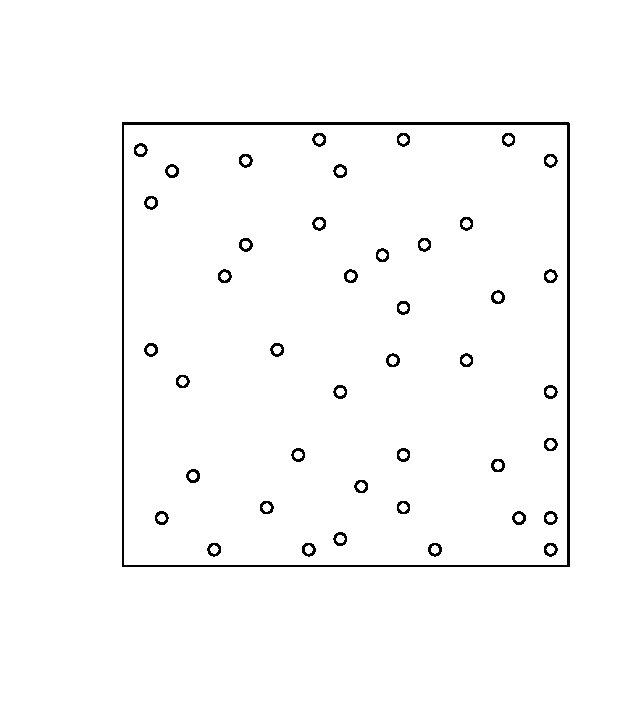
\includegraphics[width=0.49\textwidth]{DPP-in-square}
	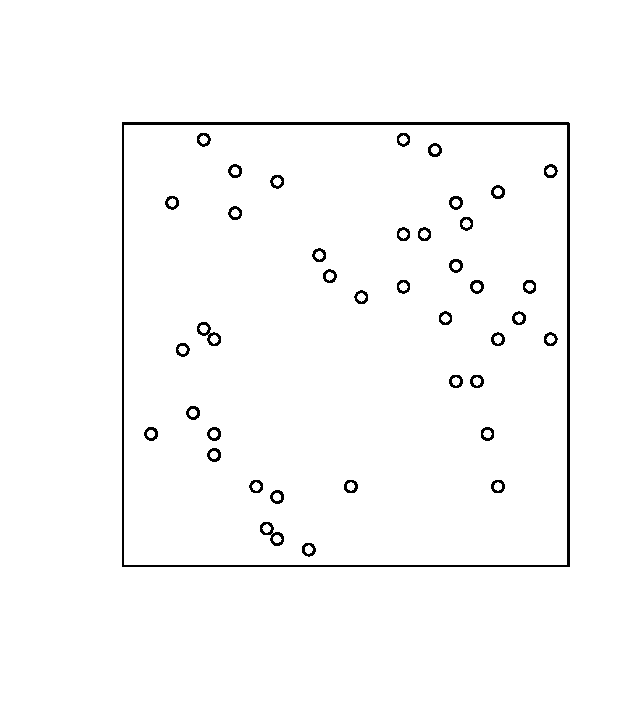
\includegraphics[width=0.49\textwidth]{Poisson-in-square}
%	\tag{1}
	\caption{A DPP with negative correlations of close points on a \(40\times40\) grid in the unit square on the left and a Poisson point process on the same grid on the right with the same expected cardinality. The -- in this case spatially -- repellent structure of the DPP is clearly visible.}
	\label{fig:1}
\end{figure}

In this light the fact that also \(\mathbf Y^c\) exhibits negative correlations becomes less surprising. Since the set \(\mathbf Y\) tends to spread out due to the repulsion in \eqref{e2.2}, the complement, which is nothing but the gaps that are left after eliminating the elements in \(\mathbf Y\), tend to show a non clustering behaviour as well.
\end{emp}

% \subsection*{\(L\)-ensembles}
\begin{emp}[\(L\)-ensembles]
Let us now introduce an important subclass of DPPs, namely the ones where not only the marginal probabilities can be expressed through a suitable kernel, but also the elementary probabilities. This will be convenient for us and lead to some explicit expression. If we have even \(K<I\), then we define the \emph{elementary kernel}
\begin{equation}\label{e2.2.1}
L\coloneqq K(I-K)^{-1}
\end{equation}
which specifies the elementary probabilities since one can check
\begin{equation}\label{e2.3}
\mathbb P(A=\mathbf Y) = \frac{\det(L_A)}{\det(I+L)} \quad\text{for all } A\subseteq\mathcal Y.
\end{equation}
Conversely for any \(L\ge0\) a DPP can be defined via \eqref{e2.2} and the corresponding marginal kernel is given by the inversion of \eqref{e2.2.1}
\[K=L(I+L)^{-1}\]
and we have again \(K<I\). We call DPPs which arise this way \(L\) \emph{ensembles}. %\todo{discuss equivalence to DPPs with \(\mathbb P(\emptyset)>0\)}
Later we will see that the cardinality of a DPP distributed like the sum of \(N\) Bernoulli experiments with expectation \((\lambda_n)_{n=1, \dots, N}\) where \(\lambda_n\) are the eigenvalues of \(K\). Being an \(L\)-ensemble is equivalent to \(K<I\) which again is equivalent to \(\lambda_n<1\) for all \(n=1, \dots, N\) and hence equivalent to
\[\mathbb P(\mathbf Y = \varnothing) = \mathbb P(\left\lvert \mathbf Y \right\rvert = 0) > 0.\]
\end{emp}

\subsection*{The quality diversity decomposition}

Note that any symmetric, positive semidefinite matrix \(L\) can be written as a Gram matrix%\todo{explain this decomposition?}
\[L=B^TB\]
where \(B\in\mathbb R^{D\times N}\) whenever \(D\) is larger than the rank \(\operatorname{rk}(L)\) of \(L\). For example one could take the spectral decomposition \(L = U^TCU\) of \(L\) and set \(B\coloneqq \sqrt{C} U\) and eventually drop some zero rows from \(\sqrt{C}\). Let \(B_i\) denote the \(i\)-th column of \(B\) and write it as the product \(q_i\cdot \phi_i\) where \(q_i\ge0\) and \(\phi_i\in\mathbb R^D\) such that \(\left\lVert \phi_i \right\rVert=1\). This yields the representation
\[L_{ij} = q_i \phi_i^T\phi_j q_j \eqqcolon q_i S_{ij}q_j\]
and we call \(q_i\) the \emph{quality} of the item \(i\in \mathcal Y\) and \(\phi_i\) the \emph{diversity feature vector} of \(i\) and \(S\) the \emph{similarity matrix}. Since we will use this decomposition multiple times, we fix its properties. % and \(S_{ij}\coloneqq\phi_i^T\phi_j\in[-1,1]\) the \emph{similarity} of the two items \(i\) and \(j\). %Further we call \(\phi_i\) the \emph{diversity feature vector} of the element \(i\).\todo{comment on \(L\) ensembles} %, which will be further explained by the later examples.

\begin{prop}[Quality diversity parametrisation]
Let \(D\in\mathbb N\) and let \(\mathbb S_D\) denote the sqhere in \(\mathbb R^D\). 
Further let \(\mathbb R^{N\times N}_{\text{sym}, +}\) be the set of symmetric positive semidefinite \(N\times N\) matrices. 
The quality diversity parametrisation is a continuous and surjective mapping %bijection
%\todo{its not a bijection!!!} %from the 
\[\Psi\colon\mathbb R_+^N\times \mathbb S_D^N \to \left\{L\in \mathbb R^{N\times N}_{\text{sym}, +} \mid \operatorname{rk}(L)\le D \right\}, \quad (q, \phi) \mapsto \left( q_i\phi_i^T\phi_j q_j\right)_{1\le i, j\le N}. \]
\end{prop}

\begin{rem}
\begin{enumerate}
\item In the case \(D = N\) the quality diversity decomposition gives a parametrisation of the whole symmetric positive definite \(N\times N\) matrices.
% \item One could argue that one should rather call the pseudo inverse of the described surection the quality diversity decomposition. However the 
\item Note that this parametrisation is not unique, i.e. \(\Psi\) is not injective. For example the identity matrix \(I\) can be parametrised by any orthonormal system \(\phi\) and \(q = (1, \dots, 1)^T\).
\item One can without any problems consider diversity features \(\phi_i\) in an abstract Hilbert space \(\mathcal H\). However we will not need this in the remainder and thus restrict ourselves to the easier case Euklidean diversity features.
\item We call every preimage \((q, \phi)\) of \(L\) under \(\Psi\) \emph{quality diversity decomposition} of \(L\). Further we call the tupel \(\phi\in \mathbb S_D^N\) of normalised vectors \emph{diversity feature matrix}.
\end{enumerate}
\end{rem}


The quality diversity decomposition will provide some useful expressions. For example the elementary probabilities take the form
\begin{equation}\label{e2.4}
\mathbb P(A=\mathbf Y) \propto \det\!\big((B^TB)_A\big) % = \det\!\big(\Psi(q, \phi)_A\big) 
= \left(\prod_{i\in A} q_i^2\right) \cdot \det(S_A) \quad \text{for all } A\subseteq\mathcal Y.
\end{equation}
% which turns out to be a very helpful expression of the elementary probabilities.%\todo{comment on advantages of choosing \(D\) small}

An intuitive understanding of the quality diversity decomposition will play a central role in the modelling process of real world phenomena through DPPs.
%later on if one wants to model real world phenomena as DPPs.
 To get this %, we can identify an item \(i\in\mathcal Y\) with the vector \(B_i=q_i\phi_i\in\mathbb R^D\) and
 we can think of \(q_i\ge0\) as a measure of how important or high in quality the item is and the diversity feature vector \(\phi_i\in\mathbb R^D\) can be thought of as some kind of state vector that consists of internal quantities that describe the item \(i\) in some way. Further we interpret the scalar product \(\phi_i^T\phi_j\in[0,1]\) as a measure of similarity between the items \(i\) and \(j\) which justifies the name similarity matrix for \(S\). Note that if \(i\) and \(j\) are perfectly similar or antisimilar, i.e. \(\phi_i^T\phi_j=\pm1\), then they can not occur at the same time, since
\[\mathbb P(i,j\in\mathbf Y) = \det\begin{pmatrix} 1 & \pm1 \\ \pm1 & 1 \end{pmatrix} = 0. \]
If we identify \(i\) with the vector \(B_i=q_i\phi_i\in\mathbb R^D\), we can obtain a geometric interpretation of \eqref{e2.4} since \(\det\!\big((B^TB)_A\big)\) is the volume that is spanned by the columns \(B_i, i\in A\), which is visualised in \ref{fig:1}. This volume increases if the lengths of the edges that correspond to the quality increase and decrease when the similarity feature vectors point into more similar directions.

%\vspace{2cm}
\begin{figure}[h!]
	\centering
	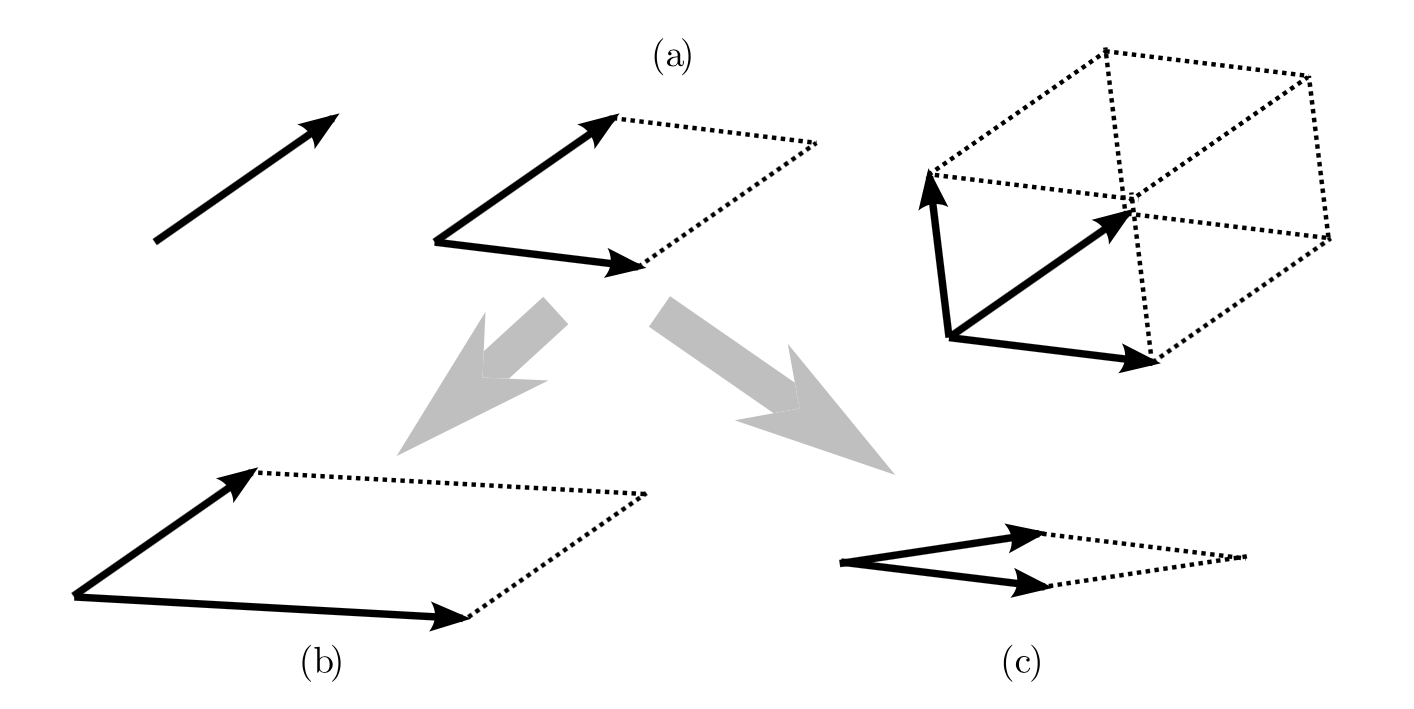
\includegraphics[width=0.8\textwidth]{qd-decomposition}
%	\tag{1}
	\caption{Taken from \cite{kulesza2012determinantal}; the first line (a) illustrates the volumes spanned by vectors, and in the second line it can be seen how this volume increases if the length -- associated with the quality -- increases (b) and decreases if they become more similar in direction which we interpret as two items becoming more similar (c)}
	\label{fig:1}
\end{figure}

\begin{emp}[Modelling diversity over distance]\label{moddiv}
Since we will use one form of diversity features multiple times, we will now give a short general formulation of it. Let \(\mathcal R = \left\{ r_1, \dots, r_D\right\}\) be a finite set which we will call the \emph{reference set} and its elements the \emph{reference points}. Further let
\[d\colon \mathcal Y\times \mathcal R\to\mathbb R_+, \quad f\colon\mathbb R_+\to \mathbb R\]
mappings. Usually \(d(i, r)\) will be interpreted as a measure of distance between an item \(i\in\mathcal Y\) and a reference point \(r\in\mathcal R\) and will typically be given by a metric on a larger space that contains both \(\mathcal Y\) and \(\mathcal R\).
One can now model \(\phi_i\in\mathbb R^{\mathcal R}\) via
\[(\phi_i)_r \propto f\!\big(d(i, r)\big) \quad \text{for } r\in\mathcal R\] % j = 1, \dots, D. \]
The function \(f\) will typically be decreasing and thus \((\phi_i)_r\) can be seen as a measure of how similar item \(i\) is to the reference point \(r\in\mathcal R\). Thus the diversity feature vector \(\phi_i\) stores how similar the item \(i\) is to all reference points and the scalar product \(\phi_i^T\phi_j\) will be close to one, if the items \(i\) and \(j\) have approximately the same degrees of similarity to the reference points. It shall be noted that the choice of the \(D\), the number of reference points bounds the rank of the kernel \(L\) and therefore of the largest subset that occurs with positive probability. Indeed we have \(\operatorname{rk}(L)\le D\) and for \(A\subseteq\mathcal Y\) with more than \(D\) elements \(\det(L_A) = 0\) and therefore \(\mathbb P(A) = 0\).
In the fourth chapter we will see that there is a natural choice for the mapping \(d\) in most cases, at least in the ones where \(\mathcal Y\) consists of %spatial positions or 
points in a metric space. On the other hand the choice of \(f\) is crucial since it determines the structure and strength of the repulsion.
\end{emp}

\begin{emp}[Transitivity of repulsion]
One last property of DPPs that we shall mention is the fact that the negative correlations of the DPP posses a transient property in the sense, that if \(i\) and \(j\) and \(j\) and \(k\) are similar, then \(i\) and \(k\) are also similar. This is due to the fact
\[\left\lVert \phi_i - \phi_j \right\rVert^2 = \left\lVert \phi_i \right\rVert^2 + \left\lVert \phi_j \right\rVert^2 - 2\phi_i^T\phi_j = 2(1-\phi_i^T\phi_j)\]
and thus
\[\sqrt{1-\phi_i^T\phi_k} = \frac12\left\lVert \phi_i - \phi_k \right\rVert\le\frac12\big(\left\lVert \phi_i - \phi_j \right\rVert + \left\lVert \phi_j - \phi_k \right\rVert\big) = \sqrt{1-\phi_i^T\phi_j} + \sqrt{1-\phi_j^T\phi_k}.\]\todo{reformulate that part!}
\end{emp}

\begin{emp}[Comparison to other point processes]

\end{emp}

% \section{\(L\)-ensembles}

\section{Variations of DPPs} %: conditional DPPs, \(k\)-DPPs and structured DPPs}

In this section we will present some useful variations of determinantal point processes. They serve different purposes and we will shortly explain their individual benefits.

%\subsection*{Conditional DPPs}

\begin{emp}[Conditional DPPs]
A \emph{conditional DPP} is a collection of DPPs indexed by \(X\in\mathcal X\), where \(X\) is called the \emph{input} of the conditional DPP. Thus for every \(X\in\mathcal X\) we get a finite set \(\mathcal Y(X)\) and a determinantal point process \(\mathbb P(\cdot\mid X)\) on \(\mathcal Y(X)\) which is given by the elementary kernel \(L(X)\), i.e.
\[\mathbb P(A\lvert X) \propto \det\left(L_A(X)\right) \quad \text{for all } A\subseteq\mathcal Y(X). \]
Further we denote the quality and diversity features of the conditional DPP by \(q_i(X)\) and \(\phi_i(X)\) respectively.

% Conditional DPPs can probably be understood the best way by giving an easy example. For this purpose we will extend our example above of the pseudo randomly selected points in a grid, but this time we don�t want to restrict ourselves to one specific grid size. Thus we will consider the input space \(\mathcal X = \mathbb N\) where the input \(n\in\mathbb N\) gives the fineness of the grid, i.e.
% \[\mathcal Y(n)\coloneqq n^{-1}\cdot\big\{ 0, \dots, n\big\}^2. \]
% So this time \(\mathcal Y(n)\) is the equally spaced grid in \([0,1]^2\) with space \(n^{-1}\) between two grid lines and we have \(N(n)=\left\lvert \mathcal Y(n) \right\rvert = (n+1)^2\).
% We model the diversities \(\phi_i(n)\in\mathbb R^{N}\) in the exact analogue way, i.e.
% \[\phi_i(n)_j \propto \left\lVert i-j \right\rVert\quad \text{for all } i, j\in \mathcal Y(n) \]
% and the explicit expressions for them remain valid.

It is not immediately clear why one would want to model a family of DPPs as a conditional DPP rather than as 
% the scenario described above by a conditional DPP rather than by a 
seperate DPPs. The reason for this is that one wants to estimate the kernels \(L(X)\) for every \(X\in \mathcal X\). However if we would do this naively we would need to observe each of the DPPs \(\mathbb P(\cdot\mid X)\) individually which is often not possible. Thus one hopes 
%The reason for this is that we hope
 to not only memorise the kernels \(L(X)\) for every single input \(X\in\mathcal X\) but rather to learn the mapping \(L\) that assigns every input \(X\) its elementary kernel \(L(X)\). If one achieved this task, one would be able to simulate and predict a DPP that one has not observed so far just by the knowledge about some DPPs that belong to the same conditional DPP. 
%  based on some training set. 
Of course this can only work if we assume some regularity or a certain structure of the function \(L\) which we will do in the third chapter where we put those consideration into a precise framework.
\end{emp}

%\subsection*{Fixed size or \(k\)-DPPs}
\begin{emp}[Fixed size or \(k\)-DPPs]

\end{emp}

%\subsection*{Structured DPPs}
\begin{emp}[Structured DPPs]
%\todo{Say something about number of parameters}
We call a DPP \emph{structured DPP} or short sDPP if the ground set is the cartesian product of some other set \(\mathcal M\), which we will call the \emph{set of parts}, i.e. if we have
\[\mathcal Y = \mathcal M^R = \left\{ y_i = (y_i^r)_{r = 1, \dots, R} \mid i = 1, \dots, N\right\}\]
where \(R\) is a natural number, \(M = \left\lvert \mathcal M \right\rvert\) and \(N = M^R\). The quality diversity decomposition of \(L\) take the form 
\[L_{ij} = q(y_i) \phi(y_i)^T \phi(y_j) q(y_j)\]
and since \(N = M^R\) is typically very big, it is impractical to define or store the quality and diversity features for every item \(y_i\in\mathcal Y\). To deal with this problem we will assume that they admit factorisations and are thus a combination of only a few qualities and diversities.

More precisely we call \(F\subseteq 2^{\left\{ 1, \dots, R\right\}}\) a \emph{set of factorisations} and for a \emph{factor} \(\alpha\in F\), \(y_\alpha\) denotes the subtupel of \(y\in\mathcal Y\) that is indexed by \(\alpha\). Further we will work with the decompositions
\begin{equation}
\begin{split}
q(y) = & \prod_{\alpha\in F}q_\alpha(y_\alpha) \\
\phi(y) = & \sum_{\alpha\in F} \phi_\alpha(y_\alpha)
\end{split}
\end{equation}
for a suitable set of factorisations \(F\) and qualities and diversities \(q_\alpha\) and \(\phi_\alpha\) for \(\alpha\in F\). Note that so far this is neither a restriction of generality -- we could simply choose \(F = \big\{\!\left\{ 1, \dots, R\right\}\!\big\}\) -- nor a simplification -- in that case we have the exact same number of qualities and diversities. However we are interested in the case where \(F\) consists only of small subsets of \(\left\{ 1, \dots, R\right\}\). For example suppose that \(F\) is the set of all subsets with one or two elements, then we only have
\[R\cdot M + \binom{R}{2} \cdot M^2 = O(R^2M^2)\]
quality and diversity features instead of
\[M^R = O(M^R).\]
This reduction of variables will make modelling, storing and estimating them feasible again in a lot of cases where naive approaches are foredoomed because of their shear size.
\end{emp}

%\begin{emp}[Sequential DPPs]

%\end{emp}

%\begin{emp}[Kronecker DPPs]

%\end{emp}

\section{Simulation and Existence of DPPs}

One of the main difficulties that arrises in the theory of discrete point processes is that they are probability measures on an exponentially large set, namely the powerset \(2^{\mathcal Y}\) which has cardinality \(2^N\). Determinantal point processes have the benefit that they describe this distribution through the matrix \(K\) which consists of only \(N^2\) parameters. This reduction of the number of parameters plays a central role in making a lot of operations possible in an computationally efficient way. However it is not only the relatively small amount of parameters that lead to this, but also the structure of the determinant itself that leads to closed expressions for a lot of quantities like the normalisation constant in \eqref{e2.3}.
In this section we will focus on the efficient simulation of DPPs and give a short overview of further techniques that can improve the performance of this algorithm.

But before we can do this we will present a famous identity for integrals -- or sums -- of the product of determinants.

\subsubsection*{Two Cauchy-Binet type formulae}

The result we present is a little technical, but we will need it later in the proof of existence and also in the proof of the sampling algorithm, so we will give the proof of it here, although it should be mentioned that all the major ideas can be found in \cite{hough2006determinantal}. In this section write \([n]\) for the set \(\left\{ 1, \dots, n\right\}\) where \(n\) is a natural number and \(A_{IJ}\) for the submatrix of \(A\) where the first index is in \(I\) and the second one in \(J\). Further we keep the notation \(A_I = A_{II}\).

%Let \([n]\coloneqq \left\{ 1, \dots, n\right\}\) further for \(I\subseteq\left\{ 1, \dots, m\right\}\) and \(J\subseteq\left\{ 1, \dots, n\right\}\) let \(A_{IJ}\) be the submatrix of \(A\) with indices in \(I\) and \(J\).

\begin{prop}[Cauchy-Binet]
Let \(m, n \in\mathbb N, m\le n\) be two natural numbers and \(A\in\mathbb R^{m\times n}, B\in\mathbb R^{n\times m}\) two matrices.  Then we have
\[\det(AB) = \sum_{\begin{subarray}{c} I\subseteq\left\{ 1, \dots, n\right\} \\ \left\lvert I \right\rvert = m \end{subarray}} \det\left(A_{[m]I}\right) \det\left(B_{I[m]}\right). \]
\end{prop}
\begin{proof}

\end{proof}�

\begin{prop}[Generalised Cauchy-Binet]\label{CB-type}
Let \(m \le n\) be two natural numbers and \(A\in\mathbb R^{m\times n}, B\in\mathbb R^{n\times m}\) two matrices. Further let \(I \subseteq[m]\), then we have
\begin{equation*}
\begin{split}
%i_{r+1}, \dots, i_{p}=1
\det\left( (AB)_{I}\right) = \sum_{\begin{subarray}{c} I\subseteq J\subseteq[n] \\ \left\lvert J \right\rvert = m \end{subarray}} \!\!\! \det\left(A_{[m]J}\right) \det\left(B_{J[m]}\right).%_{1\le k, l\le r},
\end{split}
\end{equation*}
%where\(p\le m\).
\end{prop}

\subsubsection*{Sampling and Existence}

We roughly follow the approaches taken in \cite{hough2006determinantal} and \cite{kulesza2012determinantal} and will start by showing that every determinantal point process can be seen as a mixture of a smaller class of determinantal point processes.%\todo{reference to the paper}

\begin{theo}[Mixture representation of DPPs]\label{mixDPPs}
Let \(\mathbb P\) be a DPP and \[K = \sum_{k=1}^N \lambda_kv_kv_k^T\] be the spectral decomposition of its marginal kernel. Let now \(\left\{ B_k\right\}_{k =1, \dots, N}\) be a collection of independent Bernoulli random variables with mean \(\lambda_i\). Define now the random kernel
\begin{equation}\label{BerKer}
K_B = \sum_{k=1}^N B_k v_kv_k^T.
\end{equation}
Finally define a second point process \(\tilde{\mathbb P}\) on \(\mathcal Y\) that is obtain by first drawing the Bernoulli variables \(B_k\) and then a DPP according to \(K_B\). Then we have \(\tilde{\mathbb P} = \mathbb P\) and thus \(\tilde{\mathbb P}\) is also a DPP with marginal kernel \(K\).
\end{theo}

%Before we proof this result we discuss the most important consequences.
We will postpone the proof and first discuss its consequences which will be the existence of DPPs for a given marginal kernel as well as the construction of a sampling algorithm.

\begin{rem}
Since it is fairly easy to simulate Bernoulli experiments, it remains to know how we can sample from DPPs with marginal kernels of the form \(K=\sum_{k=1}^m v_kv_k^T\) for some \(m\le N\). We call DPPs of this type \emph{elementary} and note that this corresponds to the class of DPPs where the eigenvalues of the marginal kernel are contained in \(\left\{ 0, 1\right\}\). But before we can study elementary DPPs we will fix one direct consequence of the previous theorem.
\end{rem}

\begin{cor}[Cardinality of DPPs]\label{carDPP}
Let \(\mathbb P\) be a DPP with kernel \(K = \sum_{k=1, \dots, N} \lambda_kv_kv_k^T\). Then the cardinality of the DPP is distributed like the sum of the Bernoulli variables \(\left\{ B_k\right\}_{k =1, \dots, N}\) from theorem \ref{mixDPPs}.
\end{cor}
\begin{proof}%[Proof of Theorem]
To proof this, we only have to convince ourselves that after the Bernoulli experiments the cardinality of a DPP with kernel \eqref{BerKer} has size \(m\coloneqq\sum_{k=1}^NB_k\) almost surely. Since \(K_B\) has rank at most \(k\), the cardinality is almost surely smaller than \(m\). On the other hand we have
\begin{equation}
\begin{split}
\mathbb E\big[\!\left\lvert \mathbf Y \right\rvert\!\big] = \sum\limits_{i\in\mathcal Y} \mathbb P(i\in\mathbf Y) = \sum\limits_{i\in\mathcal Y} (K_B)_{ii} = \operatorname{Tr}(K_B) = m.
\end{split}
\end{equation}
In the last step we used that the trace of a symmetric matrix is the sum over its eigenvalues, which are \(B_k\) in our case. This computation lets us conclude \(\left\lvert \mathbf Y \right\rvert = m\) almost surely.
\end{proof}

\begin{prop}[Existence of elementary DPPs]
Let \(K=\sum_{k=1}^m v_kv_k^T\) for some orthonormal set \(V = \left\{ v_k\right\}_{k=1, \dots, m}\subseteq\mathbb R^{\mathcal Y}\). Further %set \(k\coloneqq\left\lvert I \right\rvert\) and 
define the measure on \(2^\mathcal Y\) through
\begin{equation}\label{elemDPPs}
\mathbb P(A)\coloneqq \begin{cases} \; \det(K_A) \quad & \text{if } \left\lvert A \right\rvert = m \\ \; 0 & \text{else} \end{cases}.
\end{equation}
Then \(\mathbb P\) is a DPP on \(\mathcal Y\) with marginal kernel \(K\). In particular elementary DPPs exist.
\end{prop}
\begin{proof}
First we have to show that \eqref{elemDPPs} defines a probability measure. For this let \(B\in\mathbb R^{m\times N}\) be the matrix with rows \(v_k\) for \(k=1, \dots, m\). By definition we have \(K = B^TB\) and hence
\begin{equation*}
\begin{split}
\sum_{A\subseteq \mathcal Y, \left\lvert A \right\rvert = m} \det(K_A) & = \sum_{\begin{subarray}{c} I\subseteq\mathcal Y \\ \left\lvert I \right\rvert = m \end{subarray}} \det\left(K_{I}\right) %\\
%& = \sum_{i_1, \dots, i_m\in\mathcal Y} \det(B^T_{i_kl})_{1\le k, l \le m} \det(B_{i_kl})_{1\le k, l \le m} \\
 = \sum_{\begin{subarray}{c} I\subseteq\mathcal Y \\ \left\lvert I \right\rvert = m \end{subarray}} \det\left(B_{[m]I}\right)^2 \\
& = \det\left( B^TB \right) %\\
 = \det\left( v_{k}^Tv_{l} \right)_{1\le k, l\le m} = 1
\end{split}
\end{equation*}
where we have used the Cauchy-Binet identity and the fact that \(V\) is orthonormal. It remains to check that all marginal probabilities satisfy
\[\mathbb P(A\subseteq \mathbf Y) = \det(K_A).\]
For \(\left\lvert A \right\rvert\ge m\) this follows immediately, so let \(A = \left\{ i_1, \dots, i_{r}\right\}\) for \(r< m\). Then we obtain the marginal probability of \(A\) through integration over the other \(m-r\) points. Namely we have
\begin{equation*}
\begin{split}
\mathbb P(A\subseteq \mathbf Y) & = \sum_{\begin{subarray}{c} A\subseteq J\subseteq[n] \\ \left\lvert J \right\rvert = m \end{subarray}} \mathbb P(J\subseteq\mathbf Y) = \sum_{\begin{subarray}{c} A\subseteq J\subseteq[n] \\ \left\lvert J \right\rvert = m \end{subarray}} \det\left(B_{[m]J}\right)^2 %\\
% & = %\frac{(m-r)!}{m!}
%\sum_{i_r, \dots, i_m\in\mathcal Y} \det\left((v_l)_{i_k}\right)_{1\le k, l \le m}^2 = 
= \det\left( (B^TB)_A \right) = \det(K_A) % \\\det\left(K_{i_ki_l}\right)_{1\le k, l\le m} \\
%& = \frac{(m-r)!}{m!}\sum_{i_r, \dots, i_m\in\mathcal Y} \sum_{\sigma, \tau\in S_m} \operatorname{sgn}(\sigma)\operatorname{sgn}(\tau) \prod_{k=1}^{m}(v_{\sigma(k)})_{i_k}(v_{\tau(k)})_{i_k} \\% \prod_{k=r}^{m}B_{\sigma(k)i_k}B_{\tau(k)i_k}
%& = \frac{(m-r)!}{m!} \sum_{\sigma, \tau\in S_m} \operatorname{sgn}(\sigma)\operatorname{sgn}(\tau) \prod_{k=1}^{r-1}(v_{\sigma(k)})_{i_k}(v_{\tau(k)})_{i_k} \prod_{k=r}^{m} \sum_{i_k\in\mathcal Y} (v_{\sigma(k)})_{i_k}(v_{\tau(k)})_{i_k} \\
%& = \frac{(m-r)!}{m!} \sum_{\sigma, \tau\in S_m} \operatorname{sgn}(\sigma)\operatorname{sgn}(\tau) \prod_{k=1}^{r-1}(v_{\sigma(k)})_{i_k}(v_{\tau(k)})_{i_k} \prod_{k=r}^{m} v_{\sigma(k)}^Tv_{\tau(k)}.
\end{split}
\end{equation*}
where we used Lemma \ref{CB-type}.
%\todo{argue with multilinearity!}
%This expression is only non trivial when \(\sigma(k)\ne\tau(k)\) for all \(k\ge r\) and hence we can restrict the sum to those permutations that satisfy this. % which also eliminates the factor \(\frac{(m-r)!}{m!}\). Hence we get%Further we will identify 
%Further we will identify all pairs \((\sigma, \tau)\) permutations \(\)
%We obtain that this is equal to
%\begin{equation*}
%\begin{split}
%\sum_{k_1\ne\dots\ne k_{r-1}\in \left\{ 1, \dots, m\right\}} \sum_{\sigma, \tau\colon A\to \left\{ k_1, \dots, k_{r-1}\right\} \text{ bijective}} \operatorname{sgn}(\sigma)\operatorname{sgn}(\tau) \prod_{k=1}^{r-1} (v_{\sigma(k)})_{i_k} (v_{\tau(k)})_{i_k} \\
%= \sum_{k_1\ne\dots\ne k_{r-1}\in \left\{ 1, \dots, m\right\}} \det\left( (v_{k_j})_{i_l}\right)_{1\le j, l\le r-1}^2
%\end{split}
%\end{equation*}�
\end{proof}

Now we can turn towards the simulation of elementary DPPs where we will make use of the previous result.

\begin{algorithm}
\caption{Sampling from an elementary DPP \label{alg:elementary-DPP-sampling}}
\begin{algorithmic}[1]
\Require{Marginal kernel \(K=\sum_{k=1}^m v_kv_k^T\) for \(\left\{ v_k\right\}_{k=1, \dots, m}\) orthonormal}
\State \(V\gets\left\{ v_k\right\}_{k=1, \dots, m}\)
\State \(Y\gets\varnothing\)
\While{\(\left\lvert V \right\rvert>0\)}
  \State \(p_i\gets Pe_i\) the projection of \(e_i\) onto \(\operatorname{span}(V)\) for \(i\in\mathcal Y\)
  \State Select \(i\in\mathcal Y\) with probability \(\frac1{\left\lvert V \right\rvert} \cdot \left\lVert p_i \right\rVert^2\)% \sum\limits_{v\in V} (v^Te_i)^2 \)
  \State \(Y\gets Y\cup\left\{ i\right\}\)
  \State \(V\gets V_\perp\) an orthonormal basis of the subspace of \(V\) perpendicular to \(p_i\)
\EndWhile
  \State \Return{\(Y\)}
\end{algorithmic}
\end{algorithm}

\begin{prop}[Sampling from elementary DPPs]
Let \(K=\sum_{k=1}^m v_kv_k^T\), then Algorithm \ref{alg:elementary-DPP-sampling} produces a random variable \(\mathbf Y\) with values in \(\mathcal Y\) which is an elementary DPP with marginal kernel \(K\).
\end{prop}
\begin{proof}
\todo{reread!}
We note that we only have to check that \eqref{elemDPPs} holds and for this we fix \(A\subseteq\mathcal Y\). First we note that the output \(\mathbf Y\) has cardinality \(\left\lvert m \right\rvert\) since no element can be selected twice in the while loop and the size of \(V\) decreases by exactly one in each iteration. Hence it remains to show
\[\mathbb P(A = \mathbf Y ) = \det(K_A) \]
if \(\left\lvert A \right\rvert = m\). Let for the sake of convenience \(A = \left\{ 1, \dots, m\right\}\) and \(\mathcal Y = \left\{ 1, \dots, N\right\}\). Note that it suffices to show that the while loop selects \(1, \dots, m\) in this exact order with probability \(\frac1{m!}\det(K_A)\).

Let \(V_k\) denote the orthonormal set \(V\) in the \(k\)-th step of the while loop and let \(P_{k-1}\) be the projection onto \(\operatorname{span}(V_k)\) and set \(b_i\coloneqq P_0e_i\) for \(i = 1, \dots, N\). We note that if \(1, \dots, k-1\) were selected in the first steps, then \(P_{k-1}\) is exactly the projection to the subspace of \(\operatorname{span}(V_{k-1})\) that is orthogonal to \(b_1, \dots, b_{k-1}\). Since the spaces \(\operatorname{span}(V_k)\) are decreasing we have \(P_kP_j = P_k\) for \(k\ge j\) and thus \(P_{k-1} e_k = P_{k-1}P_0e_k = P_{k-1}b_k \).
 Suppose now that we have selected \(1, \dots, k-1\) in the first \(k-1\) steps of the while loop. The probability to select \(k\) in the next iteration is
\[ \frac1{\left\lvert V_k \right\rvert} \cdot\left\lVert P_{k-1}e_k \right\rVert^2 = \frac1{m-k} \cdot\left\lVert P_{k-1}b_k \right\rVert^2. \]
Thus the probability to sample \(1, \dots, m\) in this order is equal to
\[\frac1{m!} \cdot\left\lVert b_1 \right\rVert^2\cdot\ldots\cdot\left\lVert P_{m-1}b_m \right\rVert^2. \]
Since \(P_{k-1}\) is the projection onto the subspace orthogonal to \(b_1, \dots, b_k\), the product is equal to the squared \(m\)-dimensional surface measure of the parallel epiped spanned by \(b_1, \dots, b_m\). It is well known from measure and integration theory that the squared surface is given by the determinant of the Gram matrix
\[\det\begin{pmatrix}
b_1^Tb_1 & \cdots & b_1^Tb_m \\ \vdots & \ddots & \vdots \\ b_m^Tb_1 & \cdots & b_m^Tb_m
\end{pmatrix} = \det\!\big((B^TB)_A\big)\]
where \(B\in\mathbb R^{N\times N}\) is the matrix which rows are equal to \(b_k\). Therefore it remains to show \(B^TB = K^V\). However by definition \(B\) is the projection onto the span of \(V\) and thus \(B=K^V\). Because \(K^V\) is symmetric like every projection, we have \(B^T = B\) and hence can conclude \(B^TB = B^2 = B = K^V\) where we used that \(B\) is a projection.
\end{proof}

We will use Theorem \ref{mixDPPs} to prove that the following algorithm samples from a DPP. This will also show the existence of DPPs to a given marginal kernel since it gives an explicit construction.

\begin{algorithm}
\caption{Sampling from a DPP \label{alg:DPP-sampling}}
\begin{algorithmic}[1]
\Require{Eigendecomposition \(\left\{ v_k, \lambda_k\right\}_{k=1, \dots, N }\) of \(K\)}
%\Statex
\State \(J \gets \varnothing\) 
\For{\(k =1, \dots, N\)}
  \State\(J\gets J\cup \left\{ k\right\}\) with probability \(\lambda_k\)
\EndFor
\State \(V\gets\left\{ v_k\right\}_{k\in J}\)
\State \(Y\gets\varnothing\)
\While{\(\left\lvert V \right\rvert>0\)}
  \State \(p_i\gets Pe_i\) the projection of \(e_i\) onto \(\operatorname{span}(V)\) for \(i\in\mathcal Y\)
  \State Select \(i\in\mathcal Y\) with probability \(\frac1{\left\lvert V \right\rvert} \cdot \left\lVert p_i \right\rVert^2\)% \sum\limits_{v\in V} (v^Te_i)^2 \)
  \State \(Y\gets Y\cup\left\{ i\right\}\)
  \State \(V\gets V_\perp\) an orthonormal basis of the subspace of \(V\) perpendicular to \(p_i\)
\EndWhile
  \State \Return{\(Y\)}
\end{algorithmic}
\end{algorithm}

\begin{theo}[Sampling algorithm]
Let \(K\in\mathbb R^{N\times N}\) be any symmetric and positive definite matrix such that \(K\le I\). Then the distribution of the output \(Y\) of Algorithm \ref{alg:DPP-sampling} is a DPP with marginal kernel \(K\). %In particular 
\end{theo}
\begin{proof}
Theorem \ref{mixDPPs} states that an arbitrary DPP is the mixture of elementary DPPs and the for loop in the algorithm represents exactly this mixing with the respective weights. Further the sampling result for elementary DPPs yields that the output of the second part of the algorithm, namely the while loop, is distributed according to a DPP with marginal kernel \(K^V\coloneqq\sum_{v\in V} vv^T \)
%Thus we only have to show that the output of the second part of the algorithm, namely the while loop, is distributed according to a DPP with marginal kernel \(K^V\coloneqq\sum_{v\in V} vv^T \). 

%To see this let \(\mathbf Y\) denote the output and assume that \(k\) eigenvectors where selected in the first part of the algorithm and fix now \(A\).
%with \(k\) elements, where we assume for the sake of easy notation \(A = \left\{ 1, \dots, k\right\}\). 
%We seek to prove
%\[\mathbb P(A\subseteq\mathbf Y) = \det(K^V_A).\]
%However we have seen in Proposition \ref{carDPP}, that the DPP with 
%Obviously the marginal kernel \(K^V\) has rank
 %is almost surely of size
%  \(k\) and the output \(\mathbf Y\) has exactly \(k\) elements. This is due to the fact that no element can be selected twice in the while loop and the size of \(V\) decreases by exactly one in each iteration. Thus for \(\left\lvert A \right\rvert>k\) both sides are equal to zero and further for \(\left\lvert A \right\rvert<k\) we get\todo{what do we get?}
%\[\mathbb P(A\subseteq \mathbf Y) = \sum\limits_{B\supseteq A, \left\lvert B \right\rvert = k} \mathbb P(B = \mathbf Y) = \sum\limits_{B\supseteq A, \left\lvert B \right\rvert = k} \det(K^V_B) \overset{????}{=} \det(K^V_A). \]

%Thus we only have to consider the case that \(A\) has \(k\) elements %\todo{is it that simple?}{ } 
%and have to show
%\[\mathbb P(A=\mathbf Y) = \det(K^V_A).\]
%Let for the sake of convenience \(A = \left\{ 1, \dots, k\right\}\) and \(\mathcal Y = \left\{ 1, \dots, N\right\}\). 
%Since we have
% We decompose the kernel \(K^V\) as a Gram matrix \(B^TB\) which is possible just like in the quality diversity decomposition and let \(b_1, \dots, b_k\) denote the rows\todo{really?}{ } of \(B\). %and we have seen in the quality diversity decomposition that this is always possible. 
%Note that it suffices to show that the while loop selects \(1, \dots, k\) in this exact order with probability \(\frac1{k!}\det(K^V_A)\).

%Let \(V_i\) denote the orthonormal set \(V\) in the \(i\)-th step of the while loop and let \(P_{i-1}\) be the projection onto \(\operatorname{span}(V_i)\) and set \(b_i\coloneqq P_0e_i\) for \(i = 1, \dots, N\). We note that if \(1, \dots, i-1\) were selected in the first steps, then \(P_{i-1}\) is exactly 
% \(Q_i\) %\colon \operatorname{span}(V_i)\to\operatorname{span}(V_i)\) 
% the projection to the subspace of \(\operatorname{span}(V_{i-1})\) that is orthogonal to \(b_1, \dots, b_{i-1}\). Since the spaces \(\operatorname{span}(V_i)\) are decreasing we have \(P_iP_j = P_i\) for \(i\ge j\) and thus \(P_{i-1} e_i = P_{i-1}P_0e_i = P_{i-1}b_i \). % where we used that, since \(V_0\) is orthonormal, \(b_i\) is the projection of \(e_i\) onto \(\operatorname{span}(V_i)\).\todo{why?}{ }
% Suppose now that we have selected \(1, \dots, i-1\) in the first \(i-1\) steps of the while loop. The probability to select \(i\) in the next iteration is
%\[ \frac1{\left\lvert V_i \right\rvert} %\cdot \sum\limits_{v\in V_i} (v^Te_i)^2 = \frac1{k-i} 
%\cdot\left\lVert P_{i-1}e_i \right\rVert^2 = \frac1{k-i} \cdot\left\lVert P_{i-1}b_i \right\rVert^2. \]
% Here we have used that since \(V_0\) is orthonormal, \(B_i\) is the projection of \(e_i\) onto \(\operatorname{span}(V_0)\) and this implies \(P_ie_i = P_iP_0e_i = P_iB_i\). 
%Thus the probability to sample \(1, \dots, k\) in this order is equal to
%\[\frac1{k!} \cdot\left\lVert b_1 \right\rVert^2\cdot\ldots\cdot\left\lVert P_{k-1}b_k \right\rVert^2. \]
%Since \(P_{i-1}\) is the projection onto the subspace orthogonal to \(b_1, \dots, b_i\), the product is equal to the squared \(k\)-dimensional surface measure of the parallel epiped spanned by \(b_1, \dots, b_k\). It is well known from measure and integration theory that the squared surface is given by the determinant of the Gram matrix
%This surface can be parametrised by the linear mapping
%\[\Phi\colon[0, 1]^k\to\mathbb R^N, \quad e_i\mapsto b_i\]
%and the Jacobian of this is given by 
%\[\det\begin{pmatrix}
%b_1^Tb_1 & \cdots & b_1^Tb_k \\ \vdots & \ddots & \vdots \\ b_k^Tb_1 & \cdots & b_k^Tb_k
%\end{pmatrix} = \det\!\big((B^TB)_A\big)\]
%where \(B\in\mathbb R^{N\times N}\) is the matrix which rows are equal to \(b_i\). Therefore it remains to show \(B^TB = K^V\).
%, i.e. that \(B\) is the projection onto the space spanned by \(V\). 
%However by definition \(B\) is the projection onto the span of \(V\) and thus \(B=K^V\). Because \(K^V\) is symmetric like every projection, we have \(B^T = B\) and hence can conclude \(B^TB = B^2 = B = K^V\) where we used that \(B\) is a projection.
% is exactly this projection and further \(B\) is symmetric because of
%\(\det(C^TC)\) where the columns of \(C\) are \(b_1, \dots, b_k\). To see that this is equal to \(\det(K^V_A)\) we note that \(K^V = BB^T\) and set
% \[C\coloneqq \begin{pmatrix}
% I_k \\ 0
% \end{pmatrix}\in\mathbb R^{N\times k}\]
% where \(I_k\) is the \(k\times k\) identity matrix. Then we have\todo{I think there is a mistake!}
% \[\det(K^V_A) = \det(C^TBB^TC) = \det(B^TCC^TB)\ = \det(B^TB)\]
% since \(CC^T = I\).



%By definition of the surface measure this is given by\todo{check this!}
%\[\det(BB^T) = \det(K^V_A).\]

%The determinant \(\det(K^V_A)\) corresponds to the squared \(k\)-dimensional volume\todo{cite transformation theorem!}{ } of the parallel epiped that is spanned by the columns \(B_1, \dots, B_k\). This can also be expressed as
%\[\det(K^V_A) = \left\lVert B_1 \right\rVert\cdot \left\lVert P_1B_2 \right\rVert \cdot\ldots\cdot\left\lVert P_{k-1}B_k \right\rVert.\]
%Note that since \(V_0\) is orthonormal, \(B_i\) is the projection of \(e_i\) onto \(\operatorname{span}(V_0)\) and thus we have
%\[\left\lVert P_iB_{i+1} \right\rVert = \left\lVert P_ie_{i+1} \right\rVert.\]
%The second part selects \(1, \dots, k\) in this order with probability
%\[\frac1{k!}\left\lVert B_1 \right\rVert\cdot \left\lVert P_1B_2 \right\rVert \cdot\ldots\cdot\left\lVert P_{k-1}B_k \right\rVert = \frac1{k!}\det(K^V_A)\]
%what we had to show.
\end{proof}
\todo{comment on the intuition one can get from this!}

\begin{cor}[Existence of DPPs]
Let \(K\) be a symmetric \(N\times N\) matrix. Then \(K\) is the marginal kernel of a DPP if and only if \(0\le K\le I\).
\end{cor}
%\begin{proof}
%We have already seen in the beginning that this condition is necessary. To see that it is sufficient, let \(0\le K\le I\) hold. Then the point process \(\tilde{\mathbb P}\) from Theorem \ref{mixDPPs} clearly exists, for example it is given by the explicit construction in Algorithm \ref{alg:DPP-sampling} and is a DPP with marginal kernel \(K\).
%\end{proof}

We close this section with the proof of \ref{mixDPPs} given in \cite{kulesza2012determinantal}.

%\begin{lem}\label{aux}
%Let \(J\subseteq\mathcal Y\) and let \((W_n)_{n\in J}\in\mathbb R^{k\times k}\) be matrices of rank one. We denote the \(i\)-th column of \(W_n\) by \((W_n)_i\) and set \(W_J\coloneqq\sum_{n\in J} W_n\). Then we have
%\[\det(W_J) = \sum_{n_1, \dots, n_k\in J} \det\big((W_{n_1})_1(W_{n_2})_2\dots (W_{n_k})_k\big)\]%\todo{add distinct in the sum}
%where the indices \(n_1, \dots, n_k\) are distinct.
%\end{lem}
%\begin{proof}
%The multilinearity of the determinant in the columns yields
%\[\det(W_J) = \sum_{n_1, \dots, n_k\in J} \det\big((W_{n_1})_1(W_{n_2})_2\dots (W_{n_k})_k\big)\]
%and since all matrices \(W_n\) have rank one, the determinant on the right hand side vanishes if two indices \(n_i\) and \(n_j\) agree for \(i\ne j\).
%\end{proof}

\begin{proof}[Proof of Theorem \ref{mixDPPs}]
\todo{reread!}
Let %\(W_n\coloneqq v_nv_n^T\), then we have for 
\(A\subseteq\mathcal Y, k\coloneqq\left\lvert A \right\rvert\). Further set \(W_n\coloneqq (v_nv_n^T)_A\) and \(W_J\coloneqq\sum_{n\in J} W_n\). Then we have
\[\tilde{\mathbb P}(A\subseteq\mathbf Y) = \sum_{J\subseteq\mathcal Y} \det(W_J) \cdot\tilde{\mathbb P}\big(B_{i} = 1 \text{ for } i \in J\big).\]
Let \(\big((W_{n_1})_1(W_{n_2})_2\dots (W_{n_k})_k\big)\) denote the \(k\times k\) matrix with \(i\)-th row equal to the \(i\)-th row of \(W_{n_i}\). Using the multilinearity of the determinant we obtain that the marginal probability above is equal to
\begin{equation*}
\begin{split}
%\tilde{\mathbb P}(A\subseteq\mathbf Y) & = \sum_{J\subseteq\mathcal Y} \det(W_J) \cdot\tilde{\mathbb P}\big(B_{i} = 1 \text{ for } i \in J\big) \\% \prod_{i\in J} \lambda_i \prod_{i\notin J} (1-\lambda_i) \\
& % \overset{\ref{aux}}{=}
\sum_{J\subseteq\mathcal Y}\sum_{n_1, \dots, n_k\in J} \det\big((W_{n_1})_1(W_{n_2})_2\dots (W_{n_k})_k\big) \cdot\tilde{\mathbb P}\big(B_{i} = 1 \text{ for } i \in J\big) \\%\prod_{i\in J} \lambda_i \prod_{i\notin J} (1-\lambda_i) \\
 = & \sum_{n_1, \dots, n_k\in \mathcal Y} \det\big((W_{n_1})_1(W_{n_2})_2\dots (W_{n_k})_k\big) \sum_{J\supseteq\left\{ n_1, \dots, n_k\right\}} \tilde{\mathbb P}\big(B_{i} = 1 \text{ for } i \in J\big) \\%\prod_{i\in J} \lambda_i \prod_{i\notin J} (1-\lambda_i) \\
 = & \sum_{n_1, \dots, n_k\in \mathcal Y} \det\big((W_{n_1})_1(W_{n_2})_2\dots (W_{n_k})_k\big) \cdot\tilde{\mathbb P}\big(B_{n_i} = 1 \text{ for } i = 1, \dots, k\big) \\%\prod_{i = 1}^k \lambda_{n_i} \\
 = & \sum_{n_1, \dots, n_k\in \mathcal Y} \det\big((\lambda_{n_1}W_{n_1})_1(\lambda_{n_2}W_{n_2})_2\dots (\lambda_{n_k}W_{n_k})_k\big) \\
%\overset{\ref{aux}}{=}
= & \det\Big(\sum_{n\in \mathcal Y} W_n\Big) = \det(K_A).
\end{split}
\end{equation*}
%where the indices \(n_1, \dots, n_k\) are distinct.
 This computation shows that \(\tilde{\mathbb P}\) is a DPP with marginal kernel \(K\).
%In the calculation we have used the previous lemma in the second step and also in the last step where we also used the multilinearity of the determinant.
%\[\sum_{J\supseteq\left\{ n_1, \dots, n_k\right\}} \prod_{i\in J} \lambda_i \prod_{i\notin J} (1-\lambda_i) = \tilde{\mathbb P}\big(B_{n_i} = 1 \text{ for } i = 1, \dots, k\big) = \prod_{i=1}^k \lambda_{n_i}. \]
\end{proof}

%\begin{emp}[Sampling from elementary DPPs]
%\end{emp}

%\begin{emp}[Sampling from DPPs]
%\end{emp}

\subsection*{Possible improvements}

\begin{emp}[Dual sampling]

\end{emp}

\begin{emp}[Dimension reduction]

\end{emp}

\section{The mode problem}

One general motivation for modelling is the hope that predictions can be made from the selected model. If the model is of stochastic nature, like in our case, and if one wants to predict its outcome, there are a few possible approaches. The first one would be to sample from this model. This relies on the intuition that a realisation of our random variable will be a rather typical example for the random event. Going one step further one could try to find the most likely outcome of the random variable, which is known as the mode problem.

\begin{emp}[The mode problem]
Let \(X\) be a random variable with values in some space \(\mathcal X\) and let \(f\) be the density of the distribution of \(X\) with respect to some reference measure. Then the \emph{mode} is the maximiser
\[\hat x = \underset{x\in\mathcal X}{\arg\max}f(x)\]
of the density if it exists. The search for the mode is called the \emph{mode problem}.
\end{emp}

Our motivation for finding the mode of a random variable was to make better predictions for it. This is justified\todo{look for better word}{ } by the assumption that the mode should be a typical realisation of the random variable. However this is not generally the case and therefore one should be cautious with this intuition. Consider for example the mixture of two independent Gaussian random variables
\[0.1\cdot X + 0.9\cdot Y\] % \quad \text{where } X\sim N(0, 10), Y\sim N()\]
where \(X\) is centered with variance \(10\) and \(Y\) has mean \(5\) with variance \(1\), the densities are shown in Figure ....\todo{check whether this gives the desired effect and plot the density!}{ } It is clear that mode is \(0\) in this example, but it is not a very typical outcome of the random variable, since the majority of events is centered around \(10\).

The mode problem is rather well behaved if the density \(f\) is a smooth function defined on a subset of \(\mathbb R^d\), but in the case of DPPs we have to deal with the probability measure on a finite set. Thus this turns into a discrete optimisation problem over the exponentially large powerset \(2^{\mathcal Y}\). This is in general very hard to solve and it has been shown in \todo{cite} that it is NP hard to do so or even approximate it upto a factor of \(\frac89\). However there were still different strategies proposed and we will present some of them including their main ideas. \todo{do this!}



%\section{Calculations}

%\begin{enumerate}
%\item Complement of DPPs
% \item Explain why every suitably definite matrix is a marginal kernel
%\item Expression of elementary probabilities
%\end{enumerate}